\chapter{Estado del arte}
La última \textit{Encuesta de Competencias Financieras del Banco de España}, afirma que un 70\% de la población española ahorra mesualmente, pero solo un 15\% está conforme con la cantidad conseguida\cite{encuesta-competencias}. Entre los diversos métodos de ahorro conocidos encontramos el método \textit{50/30/20}, que consiste en destinar el 50\% de los ingresos a necesidades primarias, el 30\% a gastos variables y el 20\% restante a ahorro; o el método \textit{Kakebo}, que se basa en llevar un control diario de los gastos e ingresos para entender mejor el modo en que distribuimos nuestros ingresos\cite{metodos-ahorro}. Sin embargo, la falta de control sobre los gastos y la dificultad para llevar un seguimiento de los mismos, hace que muchas personas no consigan cumplir con sus objetivos de ahorro.

En este capítulo se abordarán conceptos clave relacionados con las finanzas y su impacto en la vida de las personas. Posteriormente se estudiarán las soluciones existentes en el mercado para la gestión de ingresos, gastos y ahorros con el objetivo de identificar las fortalezas y debilidades de cada una y establecer una comparativa que permita definir la propuesta de valor de la aplicación a desarrollar.

\section{Conceptos preliminares}
El uso de aplicaciones que facilitan el análisis de las finanzas personales, como la que se propone en este proyecto, motivan al usuario a tomar conciencia de cómo administra su economía y a tomar decisiones más informadas, logrando un mayor éxito en sus planes de ahorro. De este modo se abre la puerta a una mayor estabilidad financiera, y por consiguiente, a una mejora en su salud financiera. Esto nos lleva al indagar en los siguientes conceptos:

\subsection*{Finanzas personales}
Las finanzas personales son las gestiones que cada individuo realiza con su dinero 
con el propósito de satisfacer sus necesidades \cite{tesis-bienestar-financiero}.
Abarcan mucho más que el manejo e inversión del mismo, incluyen la gestión  
entendiéndose como el aprovechamiento del tiempo y dinero, que son limitados, así 
como planificaríamos un viaje debemos elaborar un plan para gestionar nuestras 
finanzas personales \cite{tyson2023personal}. 

\subsection*{Bienestar financiero}
El bienestar financiero se caracteriza por disponer de una estabilidad económica que 
permita mantener un equilibrio adecuado entre ingresos, gastos y ahorro para el futuro 
y enfrentar emergencias sin mayores dificultades. Va más allá de la acumulación de 
riqueza y se enfoca en la correcta administración del dinero, la fijación de metas 
realistas y la toma de decisiones responsables \cite{tesis-cultura-financiera}.

\subsection*{Educación financiera}
Es el proceso que ayuda a los consumidores a conocer y 
comprender mejor los productos y conceptos financieros. Según la OECD (Organización para la Cooperación y el Desarrollo Económico) con ello se fomenta el 
desarrollo de habilidades y confianza para tomar decisiones financieras informadas, ser conscientes de riesgos y oportunidades, y mejorar el bienestar financiero personal.

Su importancia radica en que permite a las personas gestionar eficientemente sus recursos, lo que contribuye a aliviar la pobreza, promover el progreso social y alcanzar un desarrollo sostenible. \textit{Una sociedad financieramente educada no solo beneficia a individuos y organizaciones, sino también fortalece la economía al hacerla más estable} \cite{capituloIX}\cite{ariza2024educacion}\cite{sarango2023educacion}.

\section{Análisis de soluciones disponibles al problema planteado}

En la búsqueda de métodos para solventar el problema de gestión, se analizan las diferentes alternativas existentes que se acercan a la solución del mismo.

\subsection{Solución tradicional}
Ya sea usando \textit{\textbf{papel y boli}}, o bien algo más 
estructurado como el uso de \textbf{hojas de cálculo}. Hay quien prefiere llevar las 
cuentas de esta manera por diversos motivos: complejidad de uso en algunas aplicaciones, 
insuficiencia de personalización para la organización de los datos, falta de entendimiento 
de la información que se representa, o simplemente por costumbre.

% \begin{table}[ht!]
%     \centering
%     \renewcommand{\arraystretch}{1.2}
%     \begin{tabular}{|p{3cm}|p{3cm}|p{3cm}|p{3cm}|}
%     \hline
%     \textbf{} & \textbf{Control de gastos} & \textbf{Gestión de ahorros} & \textbf{Resúmenes gráficos} \\ \hline
    
%     \textbf{Papel} & 
%     Responsabilidad completa sobre los cálculos para el análisis de gastos. & 
%     Planificación de ahorros y actualización del documento cuando se aporte un ahorro. & 
%     Inversión de tiempo excesiva en una tarea manual repetitiva. No automatizable. \\ \hline
    
%     \textbf{Hoja de cáculo} & 
%     Uso de recursos como fórmulas matemáticas para automatizar cálculos. & 
%     Planificación de ahorros y actualización del documento cuando se aporte un ahorro. & 
%     Inversión de tiempo en aprendizaje y creación de gráficos en la herramienta. \\ \hline

%     \end{tabular}
%     \caption{Comparación entre historial escrito en papel y hojas de cálculo}
%     \label{tab:solucion_tradicional}
% \end{table}

Estas soluciones no son las más eficientes para llevar un control exhaustivo de los gastos. La falta de automatización supone un esfuerzo extra para el usuario e inducción a errores en los cálculos, que puede llevar a la desmotivación y abandono de la tarea. Por otro lado, la falta de visualización de 
los datos en forma de gráficos dificulta la interpretación de los mismos y la toma de decisiones.

\subsection{Aplicaciones bancarias}
En la actualidad la mayoría de \textbf{aplicaciones bancarias} incorporan análisis de gastos. 
Facilitan la visualización de los movimientos de la cuenta. 

Análisis de las características más interesantes (en relación al proyecto) 
de las aplicaciones de algunos de los bancos españoles más grandes:
\footnote{\url{https://es.wikipedia.org/wiki/Anexo:Bancos_de_España}}

\begin{itemize}

    \item \textbf{CaixaBank-ImaginBank} \\
    ImaginBank es una marca comercial de CaixaBank, de los dos el primero es el banco más usado entre jóvenes. 
    En la aplicación ImaginBank, con el servicio \textit{MyMonz} \footnote{\url{https://www.imagin.com/app/mymonz}}
    se recibe un informe mensual de gastos e ingresos en la cuenta que podemos ver por categorías. 
    A diferencia de otras aplicaciones similares, no aparece la opción de 
    establecer un plan de consumo por categoría del gasto.

    En cuanto a los planes de ahorro, en el apartado \textit{Mi Hucha}
    \footnote{\url{https://www.imagin.com/ahorro/retos-ahorro}} (Figura \ref{fig:hucha_objetivo_imagin}) podemos crear 
    retos (máximo 5 huchas diferentes) con aportaciones periódicas mes a mes o de forma puntual.

    Para utilizar la aplicación es necesario ser cliente de la entidad bancaria.

    \item \textbf{Banco Santander}\\
    La aplicación del Banco Santander \footnote{\url{https://www.bancosantander.es/particulares/banca-online/apps/santander}}
    tiene una zona de \textit{Análisis de gastos}, que nos crea informes similares a los de ImaginBank. 

    Por otro lado, ésta sí nos permite establecer un 
    presupuesto por categorías que podemos revisar eventualmente para guiarnos en el 
    cumplimiento de nuestro objetivo y recibir alertas al acercarnos al límite.

    También tiene opción de ver los movimientos de compra posicionados en el mapa, aunque esta característica no funciona de manera correcta por lo que no se considera de valor en relación con el análisis de gastos. En la Figura \ref{fig:mapa_compras_santander} se localiza una compra en Barcelona, lugar donde no se realizó.

    De nuevo, es necesario ser cliente para poder usar la aplicación.\\

    \begin{figure}[ht!]
        \centering
        \begin{minipage}{0.45\textwidth}
            \centering
            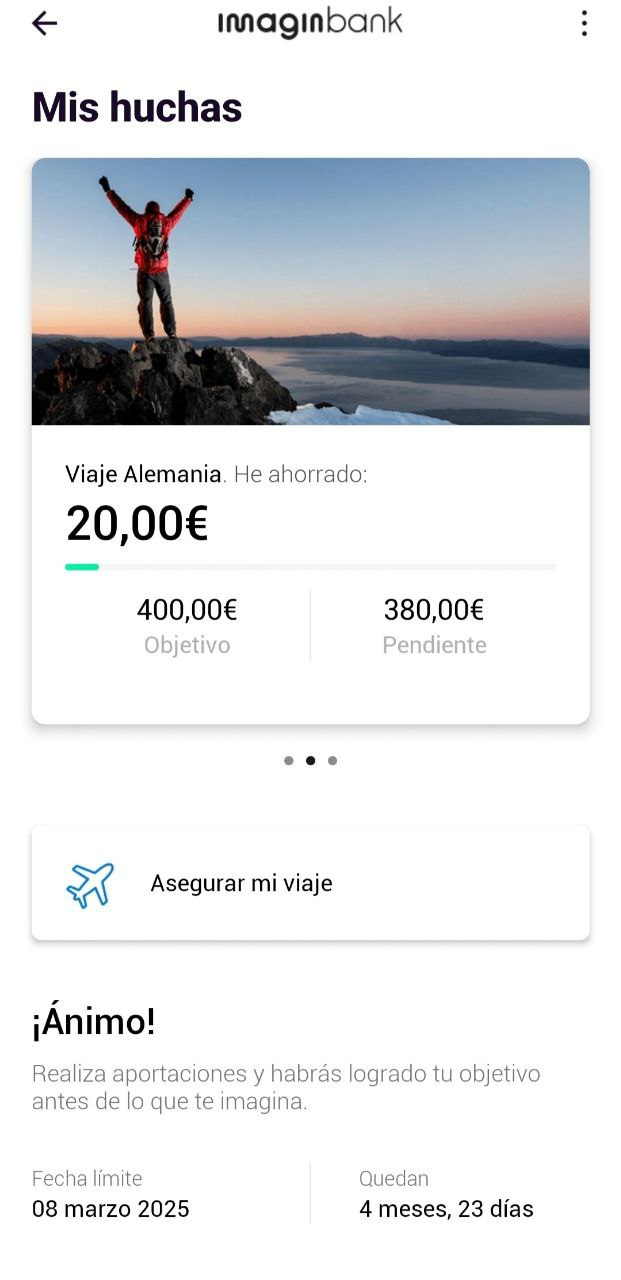
\includegraphics[height = 70mm]{imagenes/hucha-objetivo-imagin.jpg}
            \caption{Hucha de ahorro en ImaginBank\cite{hucha-imagin}.}
            \label{fig:hucha_objetivo_imagin}
        \end{minipage}\hfill
        \begin{minipage}{0.45\textwidth}
            \centering
            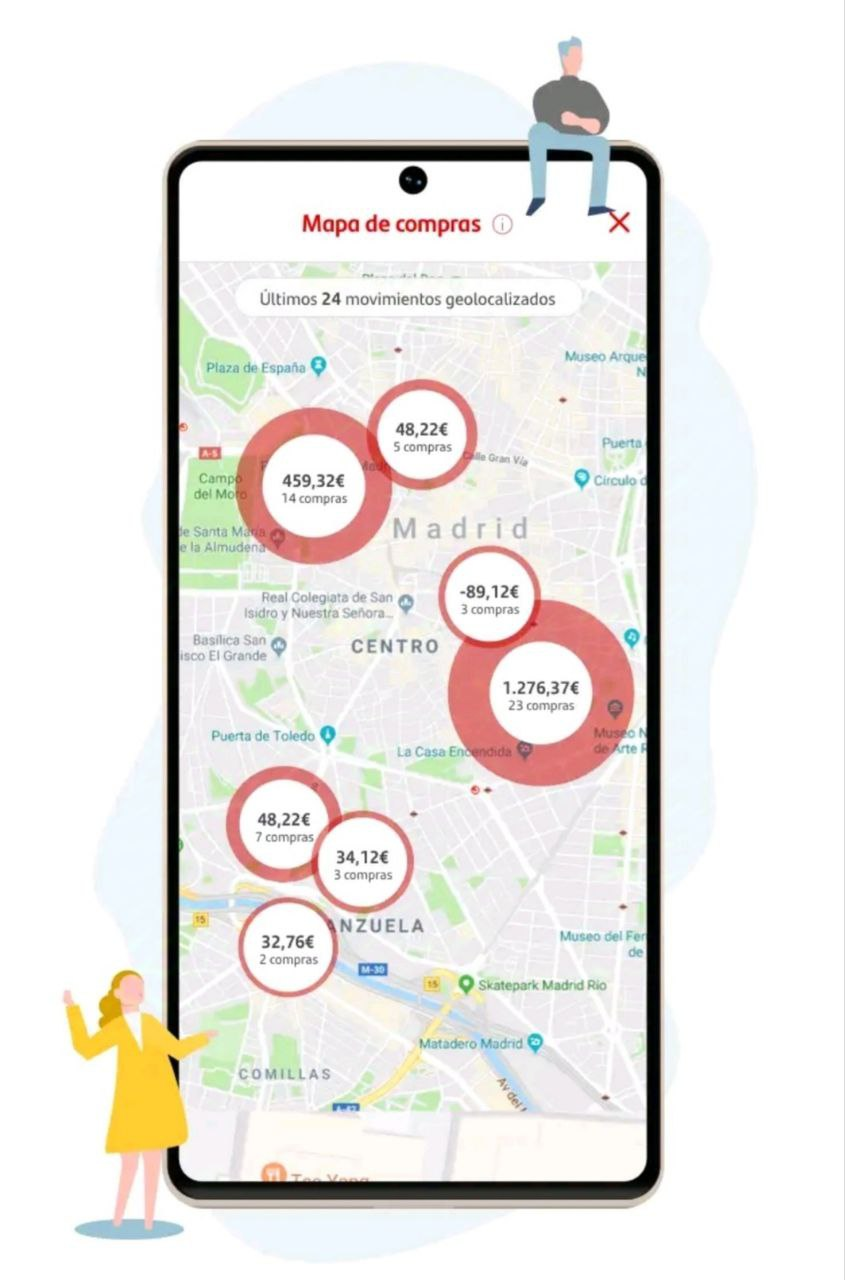
\includegraphics[height = 70mm]{imagenes/mapa-compras-santander.jpg}
            \caption{Mapa de compras en Banco Santander\cite{mapa-santander}.}
            \label{fig:mapa_compras_santander}
        \end{minipage}
    \end{figure}

    \item \textbf{BBVA}\\
    Esta última parece ser la más completa en cuanto a opciones de ahorro y análisis de gastos.

    Con \textit{Mi día a día} \footnote{\url{https://www.bbva.es/personas/banca-online/control-gastos-mi-dia-a-dia.html}}  
    obtenemos, al igual que en el resto de aplicaciones, el resumen con los movimientos de la cuenta.
    Respecto a los métodos para ahorrar existe una cuenta gratuita denominada 
    cuenta metas \footnote{\url{https://www.bbva.es/personas/productos/cuentas/cuenta-ahorro-metas.html }} 
    en la que apartar dinero a modo de hucha para conseguir hasta un máximo de 5 objetivos. 

    El apartado Presupuestos \footnote{\url{https://www.bbva.es/general/salud-financiera/economia-domestica/gestor-de-gastos-y-presupuestos.html }} 
    es el lugar donde definir una cantidad máxima de gasto deseada 
    al mes y por categoría, mide con códigos de colores la evolución del consumo 
    respecto al presupuesto (Figura \ref{fig:indicador_presupuestos_BBVA}).
    
    \begin{figure}[ht!]
    \centering
    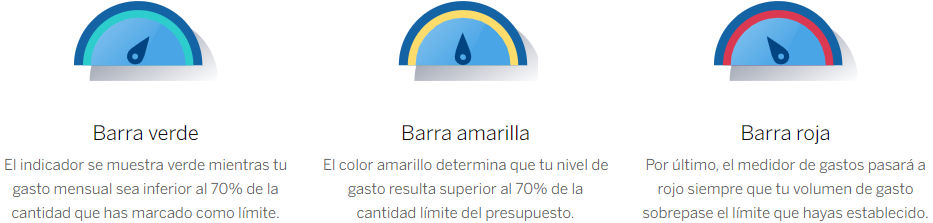
\includegraphics[height = 32mm]{imagenes/indicador_presupuestos_BBVA.png}
    \caption{Indicador de gastos respecto a presupuestos en la aplicación de BBVA
    \cite{presupuestos-BBVA}.}
    \label{fig:indicador_presupuestos_BBVA}
    \end{figure}

    Encontramos también Apartados 
    \footnote{\url{https://www.bbva.es/finanzas-vistazo/tu-guia-bbva/app/apartados-una-nueva-forma-de-ahorrar.html}}
    donde el objetivo es el mismo que en presupuestos, con la diferencia de 
    que es un espacio para separar visualmente tu dinero según tus necesidades,
    apartando la cantidad que quieras para cada tipo de gasto.

    Además, pone a disposición de los usuarios un uso parcial de la aplicación sin necesidad 
    de ser cliente, importando los datos de otros bancos (solo incluye el 
    servicio \textit{Mi día a día}).

\end{itemize}

Las aplicaciones bancarias, aunque permiten ver un resumen mensual de los gastos o incluso por categorías, en general no se pueden personalizar demasiado. Según el \textit{Estudio sobre hábitos en el uso del efectivo de 2023} publicado en el Boletín Económico del Banco de España \textit{El dinero en efectivo sigue siendo el medio de pago que mayor porcentaje de personas (65\%) usa a diario en establecimientos físicos}\cite{2023estudio-efectivo}; sin embargo, ninguna de aplicaciones anteriores permite llevar un control sobre los gastos en efectivo, lo que limita la capacidad de análisis de los gastos totales del usuario.

A pesar de que se están incluyendo opciones para importar los datos de movimientos de 
cuentas externas al banco, las configuraciones que se hacen dentro de 
la aplicación bancaria generalmente no se pueden exportar a otras aplicaciones.
Si se quiere cambiar de banco se pierde toda la información 
y con ella los planes de ahorro o presupuestos personalizados.

\subsection{Aplicaciones de terceros}
Por otro lado, existen \textbf{aplicaciones de terceros} que permiten unificar los gastos 
independientemente del banco al que pertenezca el usuario. Entre las más conocidas 
encontramos:

\begin{itemize}
    \item \textbf{Fintonic} \footnote{\url{https://www.fintonic.com/es-ES/inicio/}} \\
    El usuario agrega las cuentas bancarias que desee para que la aplicación 
    acceda a los datos relacionados con los movimientos de la cuenta. 
    Un aspecto que puede causar cierta reticencia es que para ello Fintonic necesita las claves de acceso a la cuenta bancaria (para lectura de datos).
    Recoge, clasifica y analiza los gastos por medio de gráficas y previsiones en base a meses anteriores (Figura \ref{fig:resumen_gastos_mes_fintonic}).
    Introduce los datos de manera automática por medio de las claves proporcionadas. 
    Gratuito, con publicidad.

    \item \textbf{Money Manager}  \footnote{\url{https://www.realbyteapps.com//}} \\
    Solo se encuentra disponible en inglés. Ofrece una gran cantidad de opciones
    para analizar gastos e incluye la opción de añadir fotos de las transacciones. 
    Se deben introducir los datos manualmente. 
    Dispone de una versión gratuita con funciones básicas.

    \item \textbf{Bluecoins} \footnote{\url{https://www.bluecoinsapp.com/}} \\
    Plantea una estructura interesante para mayor detalle de presupuestos. 
    Se pueden configurar presupuestos por categorías y subcategorías relacionadas, por ejemplo 
    los gastos del coche, se pueden separar en gasolina, seguro, mantenimiento, etc. 
    Permite añadir gastos manualmente o importarlos desde un archivo CSV y especificar 
    el tipo de pago si es en efectivo o digital, sin embargo no distingue de forma clara la cantidad por tipo de pago a la hora de realizar el gráfico resumen, como se puede ver en la Figura \ref{fig:resumen_gastos_bluecoins}.
    \footnote{Un fichero CSV (\textit{Comma Separated Values}) es un archivo de texto plano 
    que almacena los datos en forma de tabla, siendo cada línea del archivo una fila y 
    cada valor un campo de dicha fila. Los campos de la fila se separan entre sí por comas 
    u otro signo de puntuación.}. 
    Ofrece versión gratuita con anuncios, de funcionalidad limitada.

    \item \textbf{Mint} \footnote{\url{https://mint.intuit.com/}} \\
    Solo se encuentra disponible en inglés. Permite vincular cuentas bancarias, tarjetas, etc. para monitorizar de forma 
    automática los gastos e ingresos. Facilita la creación de presupuestos personalizados y 
    alerta al usuario cuando se acerca a sus límites de gasto.
    En base al ritmo de ahorro estima el progreso hacia el objetivo, dando recomendaciones 
    como guía para lograrlo y gestionar el dinero de manera responsable. 
    La aplicación es gratuita con algunas limitaciones e incluye publicidad.
\end{itemize}

\begin{figure}[ht!]
    \centering
    \begin{minipage}{0.45\textwidth}
        \centering
        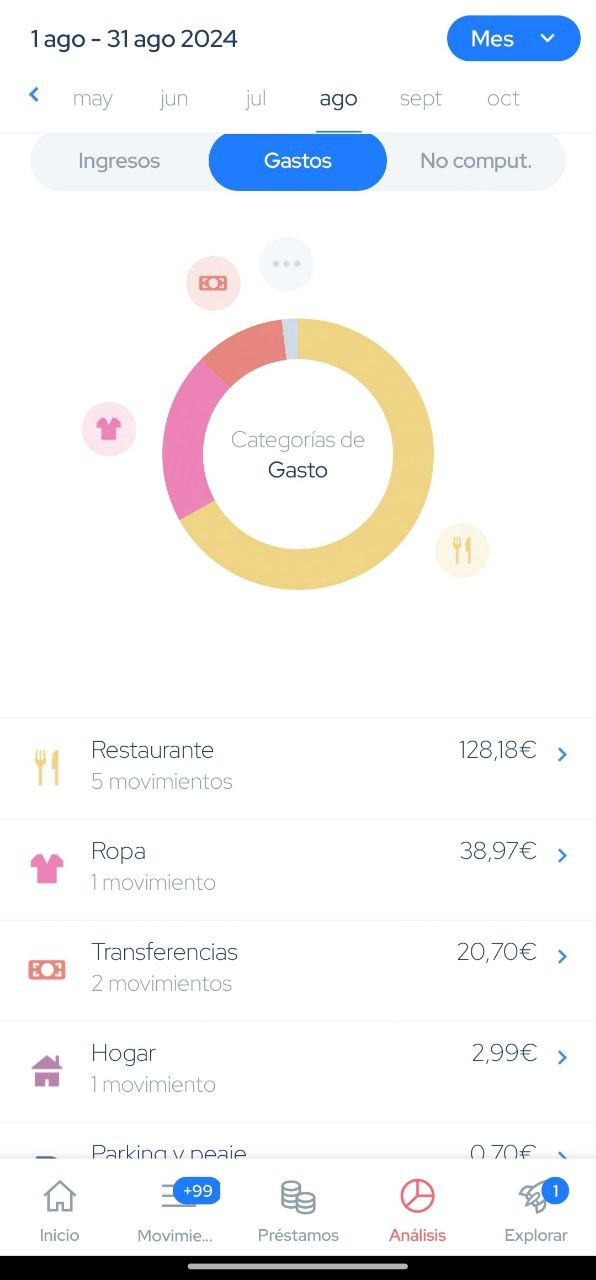
\includegraphics[height = 70mm]{imagenes/resumen-gastos-mes-fintonic.jpg}
        \caption{Resumen de gastos en Fintonic\cite{gastos-fintonic}.}
        \label{fig:resumen_gastos_mes_fintonic}
    \end{minipage}\hfill
    \begin{minipage}{0.45\textwidth}
        \centering
        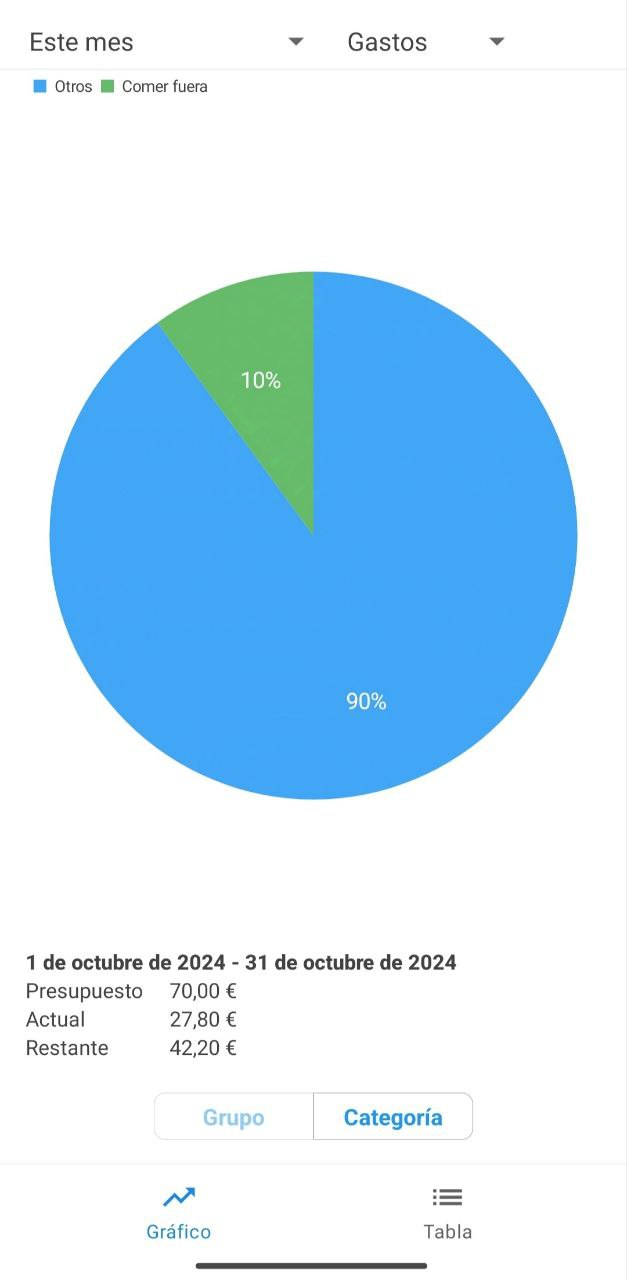
\includegraphics[height = 70mm]{imagenes/resumen-gastos-bluecoins.jpg}
        \caption{Resumen de gastos en Bluecoins\cite{gastos-bluecoins}.}
        \label{fig:resumen_gastos_bluecoins}
    \end{minipage}
\end{figure}

Además existen aplicaciones de gestión avanzada como \textbf{Pleo} 
\footnote{\url{https://www.pleo.io/es}}, que ofrece una solución para la gestión 
de gastos de empresa. Dispone de una tarjeta 
de empresa que se puede usar para pagar gastos y que se sincroniza con la aplicación 
para agilizar la contabilidad entre los empleados y la empresa. 
Entre otras características ofrece análisis útiles para el administrador en la empresa (Figura \ref{fig:resumen_gastos_pleo})
y permite a los empleados justificar los gastos al pedirles añadir foto del ticket recibido.
\begin{figure}[ht!]
    \centering
    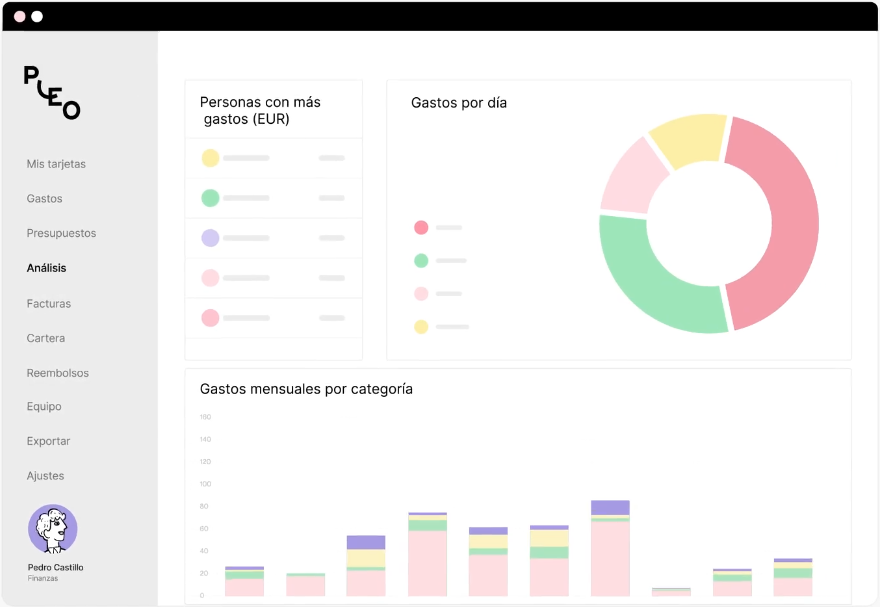
\includegraphics[width = 90mm]{imagenes/resumen-gastos-pleo.png}
    \caption{Resumen de gastos de empleados \cite{gastos-pleo}.}
    \label{fig:resumen_gastos_pleo}
\end{figure}


\subsection{Proyectos académicos}
Proyectos académicos relacionados con el ámbito de la gestión y la educación financiera.

\begin{itemize}
    \item \textbf{Sevilla Borja, Kevin Paúl}. 
    \textit{Aplicación móvil para fomentar la educación financiera en las finanzas personales 
    de los estudiantes de la PUCESA} (universidad de Ecuador) \cite{sevilla2024aplicacion}. \\
    Orientada a mejorar la capacidad
    de gestionar eficazmente las finanzas personales de los estudiantes. La aplicación 
    permite llevar un control básico de ingresos y gastos. Su característica más significativa 
    es la oferta de módulos educativos en la propia aplicación sobre conceptos financieros, como 
    ayuda para reforzar su confianza en la toma de decisiones.

    \item \textbf{Tamayo Valdivielso, Pablo}. 
    \textit{Budger: desarrollo de una app financiera} \cite{tamayo2022aplicacion}. \\ 
    Este producto desarrollado como 
    trabajo final de máster de desarrollo de aplicaciones móviles, consiste en una aplicación 
    con la que ayudar a los usuarios a controlar su dinero de una forma sencilla. Incluye 
    gráficos para visualizar el resumen de los datos y 
    permite la creación de un presupuesto global de gastos que parte del resto de los ingresos 
    que no se dedicarán a ahorro, fomentando de esta manera la planificación del usuario.

    \item \textbf{García García, Felicidad}. 
    \textit{Tus finanzas personales} \cite{garcia2019aplicacion}. \\  
    Aplicación móvil para dispositivos Android, 
    desarrollada como trabajo de fin de máster para la gestión de las finanzas personales. 
    Con finalidad de ayudar al usuario a priorizar sus gastos necesarios sobre aquellos
    que no lo son establece una clasificación de gastos en función de su importancia. 
    Los gastos se puden introducir de manera manual o permitir la incorporación de 
    movimientos bancarios accediendo a las cuentas del usuario con permiso explícito para ello.
    
\end{itemize}

\section{Conclusiones}
Tras repasar las soluciones discutidas anteriormente, encontramos numerosas 
características útiles dentro de las aplicaciones para ayudar a la gestión 
de los gastos. Algunas de ellas con más fortaleza en las secciones de análisis, 
otras en la automatización (como las que permiten la importación de datos bancarios) y  
otras, por ejemplo, en la personalización. 

Teniendo en cuenta las características generalizadas de las diferentes soluciones, 
obtenemos la siguiente tabla (Tabla \ref{tab:comparativa_soluciones}) comparativa de esfuerzo por parte del usuario.

El esfuerzo del usuario depende, en gran medida, de la aplicación y la funcionalidad concreta que necesite. Por este motivo, este proyecto surge con la idea de crear una aplicación enfocada en la gestión unificada de movimientos monetarios, para ayudar al usuario a planificar y vigilar sus gastos y ahorros independientemente de la fuente de la que provengan dichas transacciones, pero 
sin dejar de lado la automatización y personalización al incluir los datos.


\begin{landscape}
\begin{table}[]
\begin{tabular}{|l|l|l|l|l|}
\hline
& \textbf{Tradicional} & \textbf{\begin{tabular}[c]{@{}l@{}}Aplicaciones\\ bancarias\end{tabular}} & \textbf{Aplicaciones de terceros} & \textbf{\begin{tabular}[c]{@{}l@{}}Proyectos\\ académicos\end{tabular}} \\ \hline
\textbf{\begin{tabular}[c]{@{}l@{}}Anotación de movimientos\\ (gastos, ingresos y ahorros)\end{tabular}} & Alto & Muy bajo & \begin{tabular}[c]{@{}l@{}}Con integración banco: Muy bajo\\ Sin integración banco: Medio - Alto\end{tabular} & Medio - Alto \\ \hline
\textbf{Control de dinero efectivo} & Alto & No tienen & \begin{tabular}[c]{@{}l@{}}Con integración banco: No tiene\\ Sin integración banco: Medio\end{tabular} & Medio \\ \hline
\textbf{Control de dinero digital} & Alto & Bajo & Bajo & Bajo \\ \hline
\textbf{\begin{tabular}[c]{@{}l@{}}Creación de categorías de\\ gastos (con presupuestos)\end{tabular}} & Alto & \begin{tabular}[c]{@{}l@{}}No personalizable\\ (automático)\end{tabular} & Medio - Bajo & Bajo \\ \hline
\textbf{\begin{tabular}[c]{@{}l@{}}Creación de objetivos de\\ ahorro\end{tabular}} & Alto & \begin{tabular}[c]{@{}l@{}}Bajo (nº limitado\\ de objetivos)\end{tabular} & \begin{tabular}[c]{@{}l@{}}Con integración banco: No tienen\\ Sin integración banco: Medio\end{tabular} & \begin{tabular}[c]{@{}l@{}}No tienen (lo que no\\ se gasta se considera\\ ahorro)\end{tabular} \\ \hline
\textbf{Resúmenes de gastos totales} & Alto & Muy bajo & Muy bajo & Muy bajo \\ \hline
\textbf{\begin{tabular}[c]{@{}l@{}}Representación gráfica\\ de gastos\end{tabular}} & Medio - Alto & Muy bajo & Muy bajo & Muy bajo \\ \hline
\textbf{\begin{tabular}[c]{@{}l@{}}Representación gráfica\\ de ahorros\end{tabular}} & Medio - Alto & No tienen & Muy bajo & Muy bajo \\ \hline
\textbf{Personalización} & Bajo & Medio - Alto & \begin{tabular}[c]{@{}l@{}}Con integración banco: Alto\\ Sin integración banco: Medio\end{tabular} & Bajo \\ \hline
\end{tabular}
\label{tab:comparativa_soluciones}
\caption{Comparativa de esfuerzo por parte del usuario en las diferentes soluciones.}
\end{table}
\end{landscape}

